\chapter{$\dzero$~Level3 Trigger and Data Acquisition System}
\label{Level3}

\section{Introduction}

$\dzero$~utilizes a three level trigger system to reduce the data rate from 1.7~MHz to 50~Hz. The first trigger level reduces the rate to 1.5~kHz by selecting events based on calorimeter energy, hits in the muon system, or tracks in the CFT. The level 2 trigger reduces the rate to 800~Hz using sub-detector specific pre-processing boards to select events with electrons, muons, and jets. If the event satisfies the level 1 and level 2 trigger, the sub-detector data is readout and stored in memory on single board computers (SBC) located in the detector VME crate module. The SBC data is transmitted over ethernet and routed to one in a collection of farm nodes, which execute the level 3 trigger decisions. If the event satisfies the level 3 it is recorded to tape. 

The following section describes the hardware and software components in the L3/DAQ system. The single board computers which interface with the VME crate data are described in Section~\ref{l3-sbc}. A dedicated SBC called the Routing Master is employed to route data stored on the SBCs based on the availability of the farm to process the event. The Routing Master and its routing software is described in Section~\ref{l3-rm}. A large ethernet switch capable of transmitting $\sim16$~GB/s is used to route the SBC data to its associated farm node. This switch and the data path over ethernet cables is described in Section~\ref{l3-eth}. The farm nodes and the software which collects event fragments from each sub-detector crate are described in Section~\ref{l3-farm}. A softwa

The following section describes the L3/DAQ system in more detail. Section~\ref{l3-hardware} describes the hardware compone

The L3 trigger 
The $\dzero$~data acquisition and L3 trigger system is designed to record and process data from each sub-detector to select events for tape storage.

\section{Hardware}
\label{l3-hardware}

\section{Farm Node}
\label{l3-farm}

\section{Ethernet Switch}
\label{l3-eth}

\section{Routing Master}
\label{l3-rm}

\section{Single Board Computer}
\label{l3-sbc}

\begin{itemize}
\item readout controllers for sub-detector data
\item VMIC 7750 - PIII 933 MHz with 128~MB of RAM and 128~MB of flash memory.
\item 

\subsection{Farm Node}

\subsection{Ethernet Switch}

\section{Software}

\section{Monitoring}

\begin{figure}[!h!tbp]
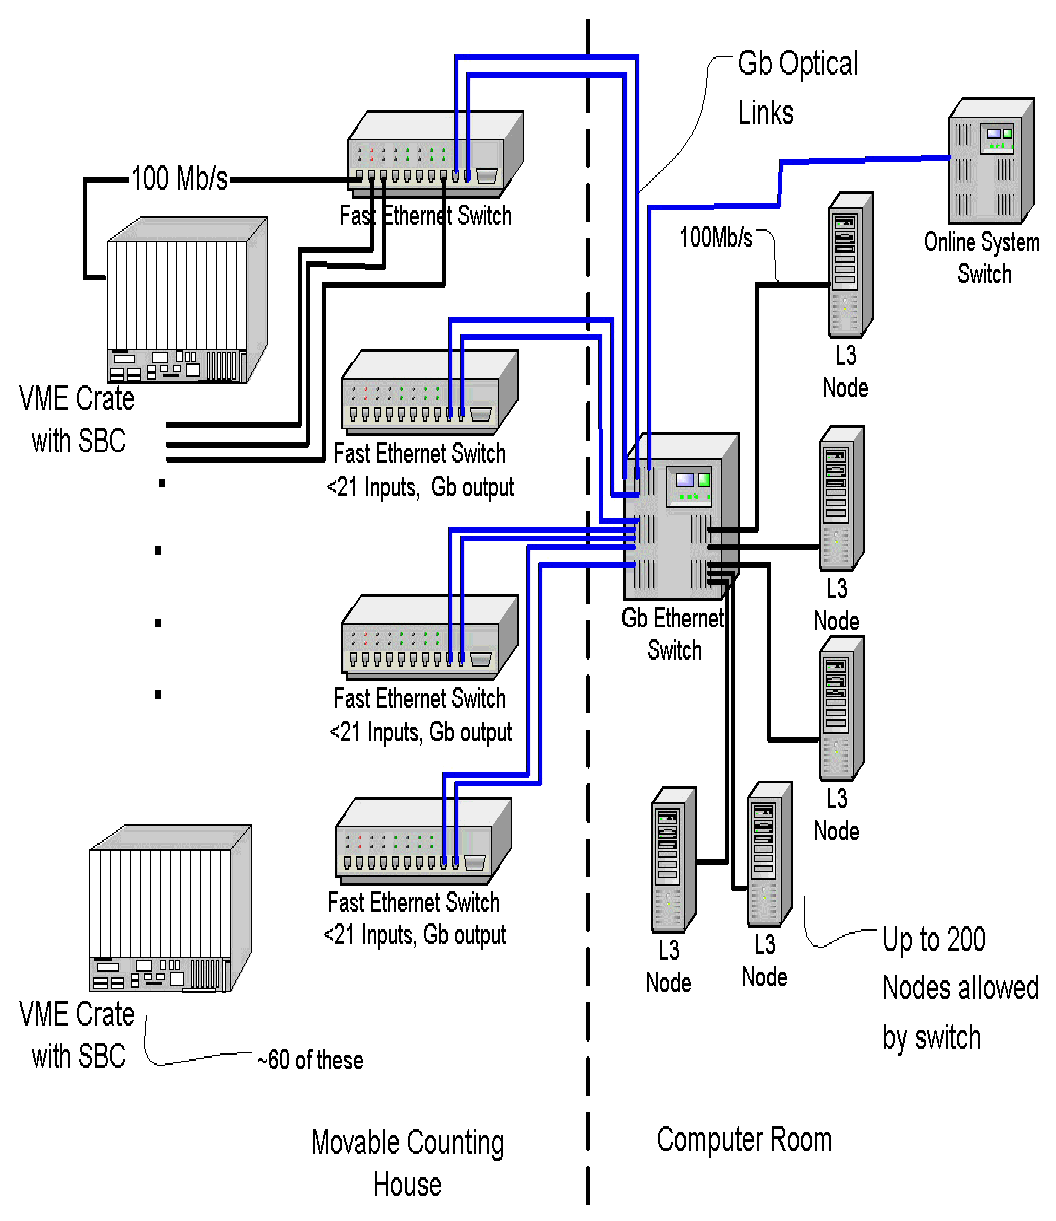
\includegraphics[width=0.49\textwidth]{eps/Level3/L3-DAQ.eps}
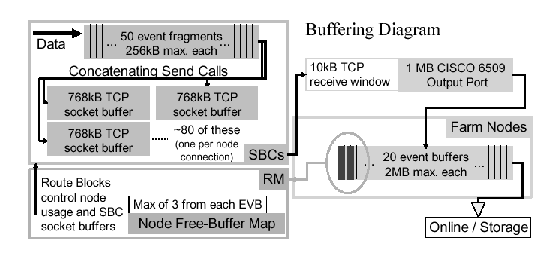
\includegraphics[width=0.49\textwidth]{eps/Level3/buffering.eps}
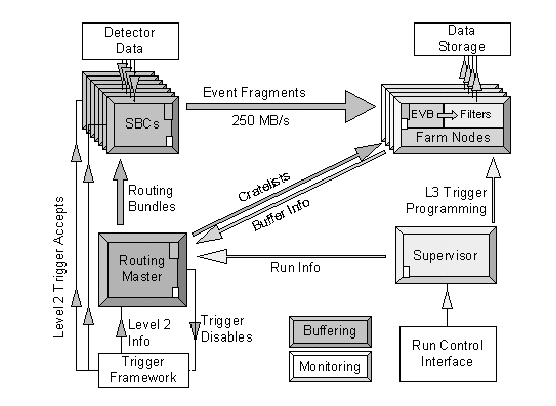
\includegraphics[width=0.49\textwidth]{eps/Level3/daq_software.eps}
\vspace{-0.1in}
\caption{Measured 1D posterior plots for the combined
$e$+$\mu$ $\geq$~1 $B$-tag channel with statistical uncertainties only
(left plot) and with systematic uncertainties as well (right plot).}
\label{meas-post-1d}
\end{figure}
